\scanpage{32}
\uline{Ex. 2} Soit $C$ comme dans Ex. 1 et soit $\unsure{\mathcal D|\mathcal P}$ une catégorie de Deuring reliée à $A$. Un \uline{foncteur norme} de $C$ à $\unsure{\mathcal D|\mathcal P}$ est un couple $(\nu,\alpha)$, où
\[
\nu:C\longrightarrow D\qquad\text{un foncteur (en général pas additif!)}
\]
\[
\alpha=(\alpha_{X,P}):\nu(P\otimes_O X)\xrightarrow{\sim}
\underbrace{\operatorname{Nr}_{O/A}}_{\text{norme réduite}}(P)\otimes_A\nu(X)
\]
un système d'isomorphismes, satisfaisant les conditions de transitivité, et fonctorialité en $P,X\ldots$.

\margin{\unsure{Généraliser} au cas où $\unsure{D|\mathcal P}$ n'est pas néc. de Deuring, mais seulement \inserted{$A$-lin.} \unsure{que les} $\operatorname{Nr}_{O/A}(P)\otimes_A Y$ $(Y\in\operatorname{Ob}\unsure{D|\mathcal P})$ existent.
\figure{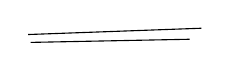
\begin{tikzpicture}[x=1cm,y=1cm]\draw (0,0)--(2.2,.08);\draw (.03,-.10)--(2.05,-.06);\end{tikzpicture}}
Montrer qu'il y a une $D$ universelle recevant un foncteur norme, \unsure{qu'on écrira} $V_A(C)$. \deleted{$\unsure{N_{A/K}(C)|N_A(C)}$} Noter que $V_A(C)$ commute aux chgts de base du type envisagé en Ex. 1 \deleted{\unsure{ce qui est}}.}

\deleted{Pour} \unsure{Si} $X$ fixé dans $\operatorname{Ob}C$, la cat. des foncteurs \deleted{déterminants}\inserted{normes} est \inserted{can.} équiv. \deleted{can.} à celle des objets $T_0$ de $\unsure{D}$, en définissant $\nu$ par
\[
\nu(P\otimes_O X)\simeq\operatorname{Nr}_{O/A}(P)\otimes T_0.
\]
\diagram{\begin{tikzcd}
\deleted{C}\arrow[r,"\deleted{(\nu,\alpha)}",crossing over]&\deleted{D}
\end{tikzcd}}
Supposons maintenant qu'on ait un isom fonctoriel en $P\in\mathbb P(O/A)$
\[
\operatorname{Nr}_{O/A}(P)\simeq A
\]
\margin{avec conditions de transitivité\ldots \unsure{compatibilités}}
\diagram{\begin{tikzcd}
\deleted{A}\arrow[r,rightsquigarrow]&\deleted{\unsure{A}}
\end{tikzcd}}
\margin{Noter qu'alors la catégorie $V_A(C)$ est munie d'une section canonique $\tau$ et $\nu_C$ est \unsure{c\textsuperscript{te} v.l.} $\tau$.}
Soit $A'\mathbin{-}A$ un chgt de base du type envisagé dans ex. 1, et considérons \deleted{$\unsure{E}$} sur $A'$ des catégories de Deuring $C',D'$, et un hom norme $(\nu,\alpha):C'\mathbin{-}D'$. Soit enfin $\varphi:C\mathbin{-}C'$ un foncteur admissible.
\diagram{\begin{tikzcd}
C\arrow[r,"\varphi"]&C'\arrow[r,"\nu"]&D'\\
A&A'&
\end{tikzcd}}
Alors \deleted{\unsure{p}} on a un objet can. $T_\varphi$ de $D'$, et un isom $\nu(\varphi(X))\simeq T_\varphi$.
\mspage{31}
